\chapter{Development}

\section{Hardware Design}
The hardware of the Fleet-Monitor was design using Altium Designer 21. The integrated 3D \acrshort{cad} functionality simplified the overall development and lowered the chance of errors in the design. The 4-Layer \acrfull{pcb} with the size of 140.5 mm x 79.5 mm has been manufactured and assembled by JLCPCB.\newline
As a proof of concept, five prototypes have been made, which are all fully tested and in working condition.

\todo{Add Rendering of PCB only}
\medskip
\begin{figure}[h!]
	\centering
	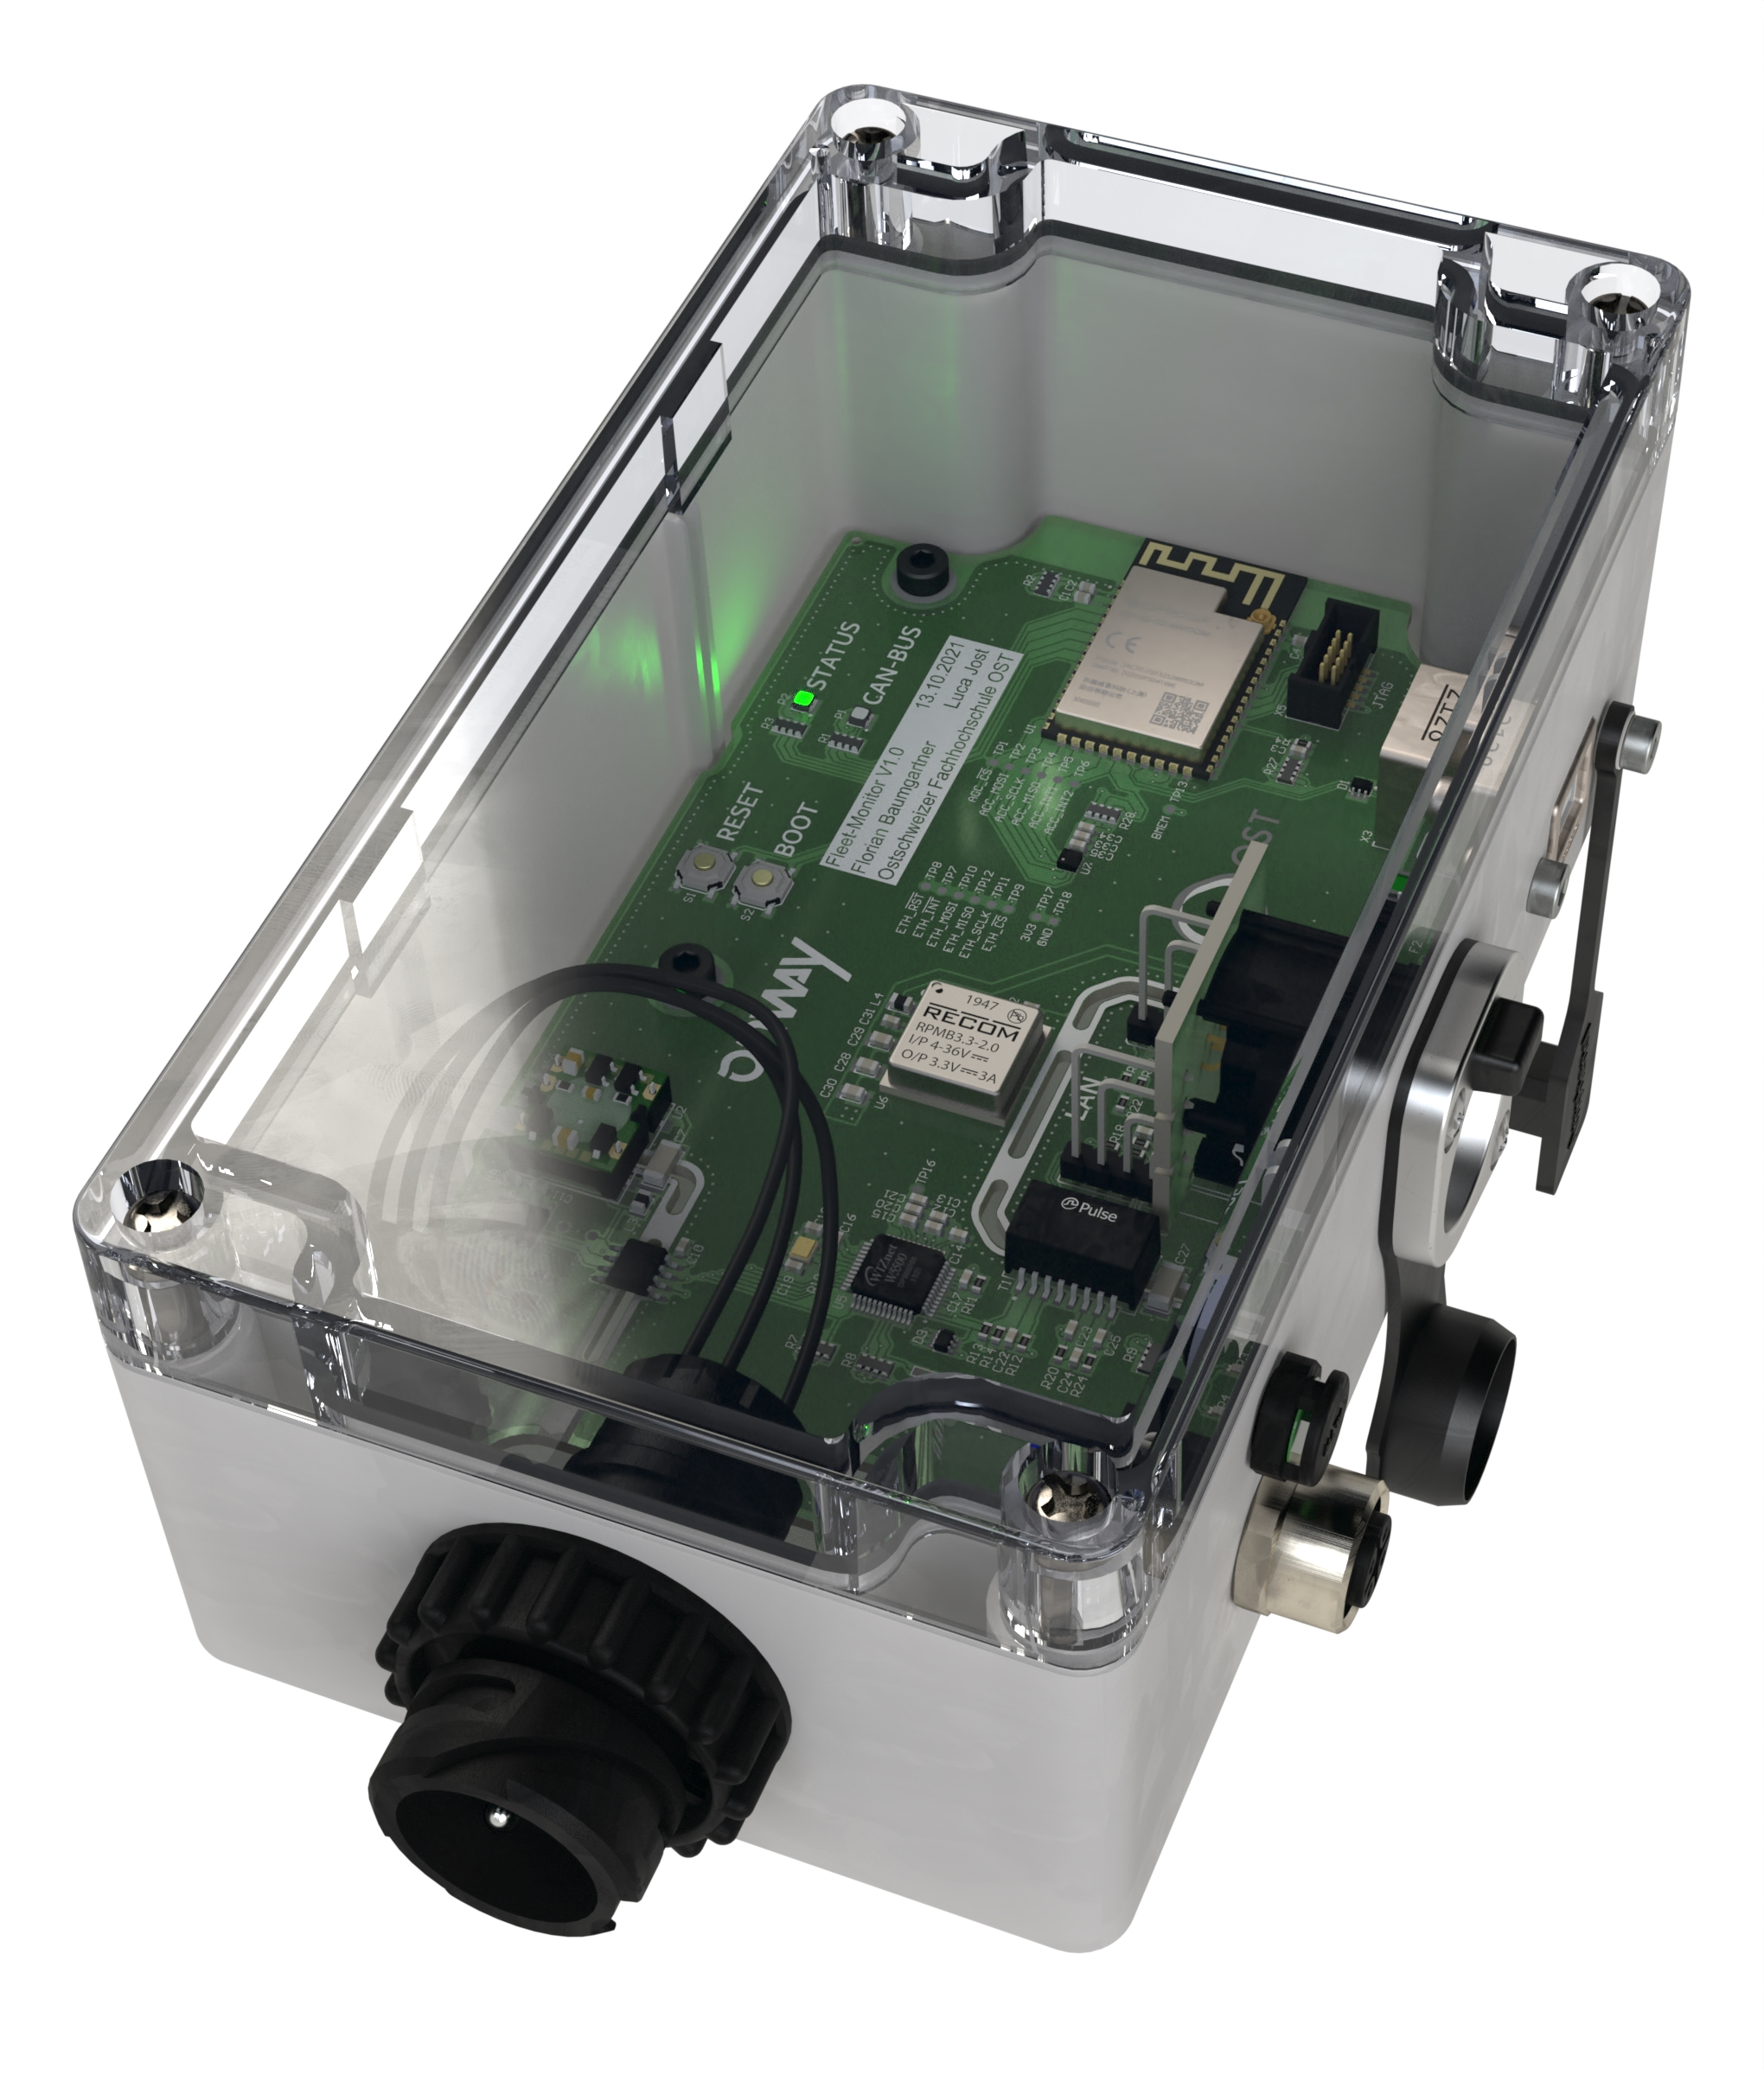
\includegraphics[height=9cm]{images/fleet-monitor-rendering}
	\caption{Assembled PCB 3D-Render}
	\label{fig:fleet-monitor-rendering}
\end{figure}

\subsection{Power Management}
The device can be powered ether by the \acrshort{usb}-Interface or an external DC power source. Both supply options are internally connected through Schottky diodes and provide a seamless switch-over. If both supply sources provide power at the same time, the external one gets preferred.\newline
The \acrfull{usb} Interface fulfills all guidelines of the \acrshort{usb} specifications in terms of power consumption. Therefor it is guaranteed, that the maximal current of 500 mA is not exceeded. In case of failure, a resettable \acrshort{ptc} Poly-fuse protects the power source of potential over current.\newline
The external power source accepts a voltage range from 9 V to 28 V and is protected against wrong polarization and short circuit. As a suitable connector, the industry standard M12 (5 Pin) type has been chosen. It fulfils the IP67 rating and is highly robust against accidental disconnection due to its threaded coupling. In addition it is used in a wide variety of applications, resulting in great availability. The pin-out consists of pin 1 and 2 used for the positive input and pins 3 to 5 for ground. This has the advantage, that matching connectors with a different amount of pins (e.g. 2-pin connector) can be used as well.\newline
The core of the power management unit is based on a Recom DC-DC converter of the RPMB-2.0 series. The very compact design, great performance and fairly low price offers an optimal solution.\newline
The total power consumption of the device is in average around 1.5 W.

\todo{Add PTC Fuse in fron of diode in diagram}
\begin{figure}[h!]
	\centering
	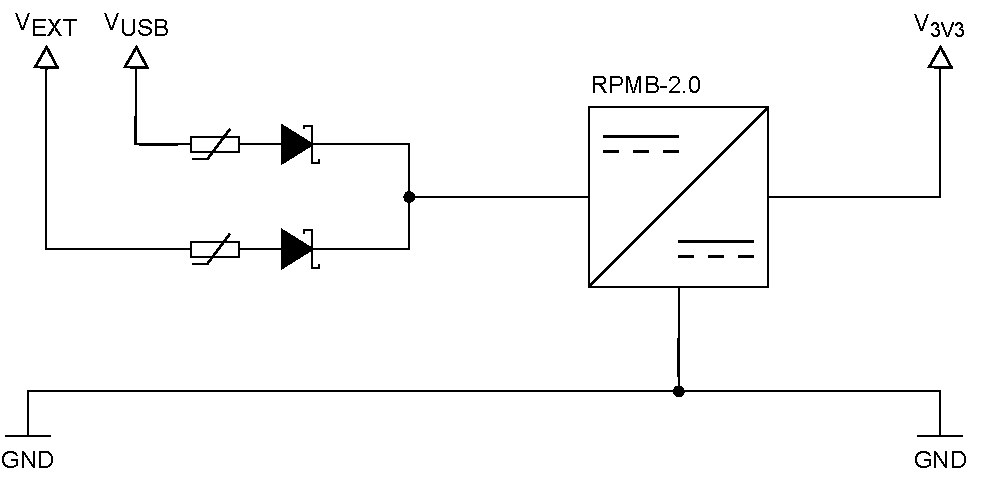
\includegraphics[height=5cm]{images/power}
	\caption{Simplified Power Management}
	\vspace{-1.4ex}
	\label{fig:simplified-power}
\end{figure}
\newpage

\subsection{ESP32-S2}
The choice of a suitable micro controller is crucial in the design of an embedded system. Several factors were carefully considered and key requirements have been set, such as:

\begin{itemize}
		\item Integrated Wi-Fi subsystem and \acrshort{rf} front-end
		\item System performance: CPU speed, memory and peripherals
		\item Native \acrshort{usb} 2.0 Interface
		\item Physical package and pin count
		\item Availability (especially in an ongoing worldwide chip-shortage)
\end{itemize}

The Espressif's \gls{esp32} \acrfull{soc} family satisfies all listed requirements and is in addition advertised as a low cost solution.\newline
To reduce design complexity and production cost, the ESP32-S2 has been embedded as a solder-on module of the type ESP32-S2-WROOM-I. This module has the advantage of containing the RF front-end inclusive an integrated \acrshort{pcb} antenna as well as a 4 MB \acrshort{spi} flash chip.\newline

%\medskip
\begin{figure}[h!]
	\centering
	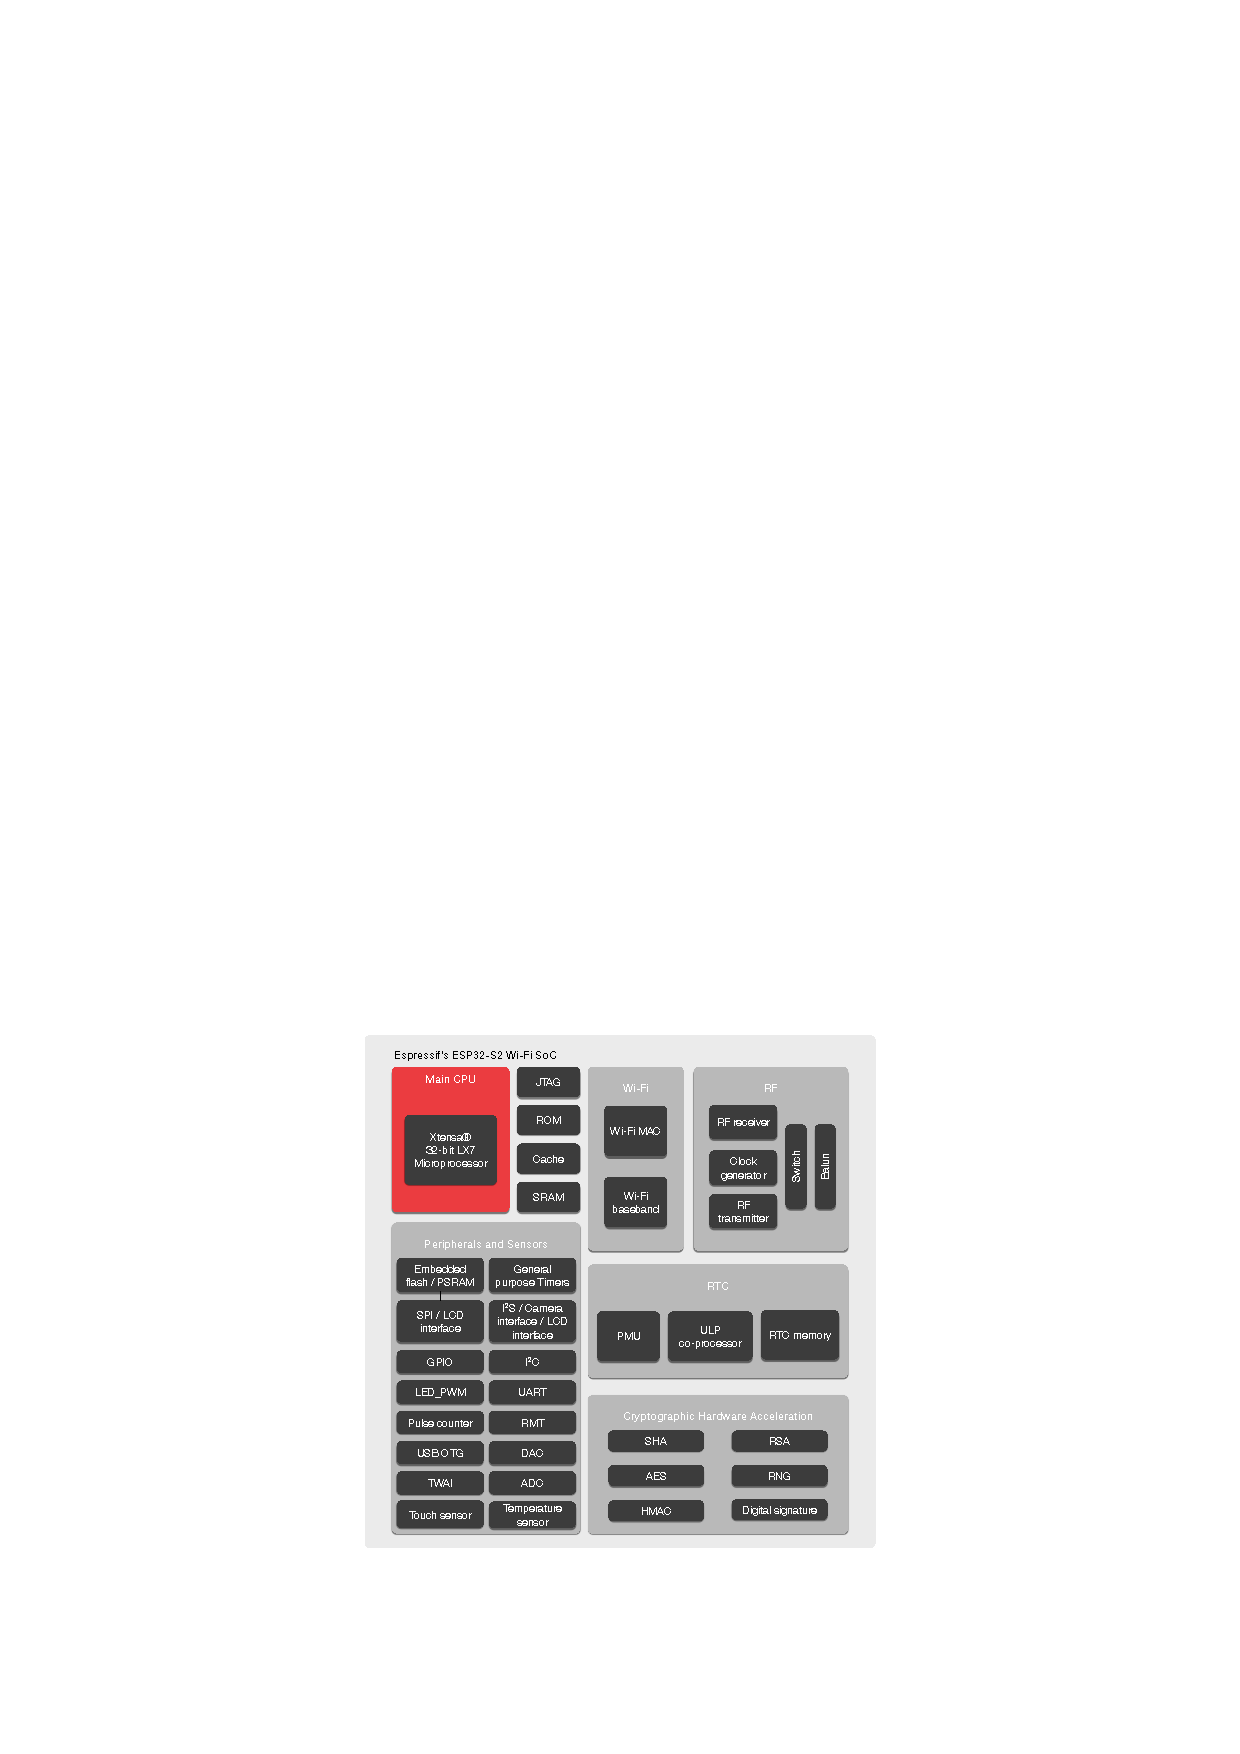
\includegraphics[height=9cm]{images/esp32-s2_block_diagram}
	\caption{ESP32-S2 Block Diagram}
	\vspace{-1.4ex}
	\caption*{\textbf{Source:} ESP32-S2 Datasheet \cite{esp32-s2_datasheet}}
	\label{fig:esp32-s2_block_diagram}
\end{figure}

The \acrshort{soc} can be programmed ether by \acrshort{jtag} and a suitable programmer (e.g. Espressif's ESP32-Prog) or conveniently over the integrated \acrshort{usb}-Interface.\newline
For uploading code via the \acrshort{usb}-Interface, the ESP32-S2 has to be set in to the device firmware update mode. This can be achieved by pressing the boot button while the device is booting (e.g. after powering on or a reset). If the boot button is not accessible, the user can force the device to enter the \acrshort{dfu} mode by setting a flag in the system configuration. This procedure gets further explained in the user manual section.\newline
\newpage

\subsection{Ethernet Interface}
The Ethernet interface utilizes a WIZNet W5500 Ethernet controller chip with an integrated \acrshort{phy} and \acrshort{tcp/ip} stack. It is capable of transmission speeds of 10 or 100 MBit/s. The chip is connected through \acrshort{spi} with the main processing unit (\gls{esp32}).
The IEEE standard 802.3 specifies a 1500 V\textsubscript{RMS} isolation barrier between the Ethernet PHY Chip and the cable. To comply with these requirements a pulse transformer was used to magnetically couple the data lines between the connector and the chip. Additionally a ground clearance of \todo{add distance} mm was chosen to avoid flash over or tracking between electrical conductors as seen in \todo{add image}. 

\begin{figure}[h!]
	\centering
	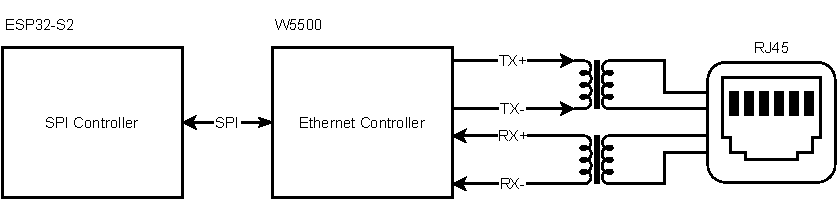
\includegraphics[height=2.5cm]{images/eth_interface}
	\caption{Simplified Ethernet Interface}
	\vspace{-1.4ex}
	\label{fig:eth-interface}
\end{figure}

\todo[inline]{Write about Ethercon ® connector}

\begin{figure}[h!]
	\centering
	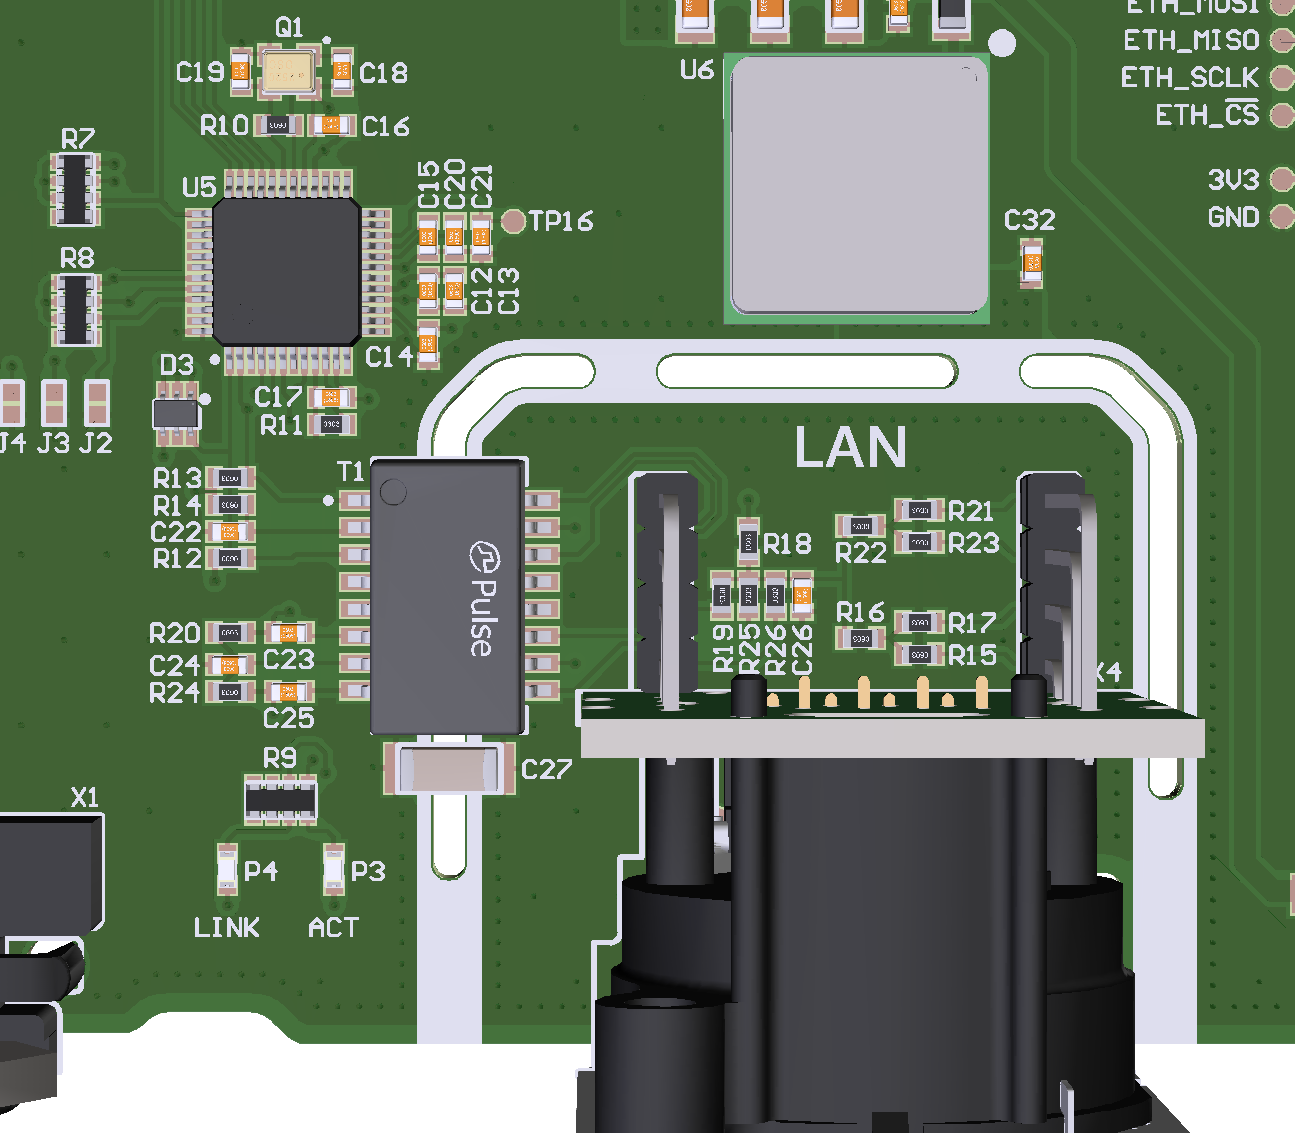
\includegraphics[height=7cm]{images/eth-pcb}
	\caption{PCB view of Ethernet Interface}
	\vspace{-1.4ex}
	\label{fig:eth-pcb}
\end{figure}

\newpage

\subsection{CAN-Bus Interface}
The \acrfull{twai} is a real-time serial communication protocol suited for automotive and industrial applications. It is compatible with CAN bus frames following the ISO11898-1 standard. The ESP32-S2 contains a \acrshort{twai} controller that can be configured to communicate on a CAN bus via an external transceiver.

\begin{figure}[h!]
	\centering
	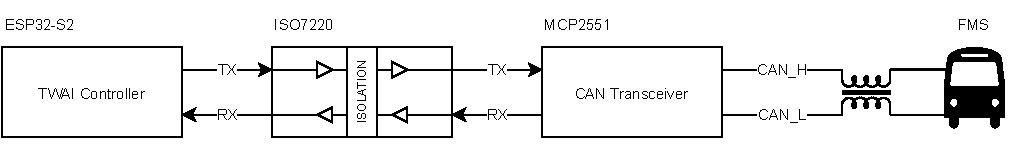
\includegraphics[height=1.8cm]{images/can-interface}
	\caption{Simplified CAN Interface}
	\vspace{-1.4ex}
	\label{fig:can-interface}
\end{figure}

\subsubsection{Transceiver}
The data lines are translated using a CAN transceiver from Microchip (MCP2551). The role of the transceiver is to drive and detect data to and from the bus. It converts the single-ended logic used by the controller to the differential signal transmitted over the bus. The MCP2551 device provides transmit and receive capabilities and is fully compatible with the ISO-11898 standard. \newline

\subsubsection{Isolation}
A dual-channel digital isolator (ISO7221BDR) was used in conjunction with an isolated DC/DC converter from Recom (R1SX-3.305/H). These devices block high voltage and isolate grounds, as well as prevent noise currents on a data bus or other circuits from entering the local ground and interfering with or damaging sensitive circuitry.

\begin{figure}[h!]
	\centering
	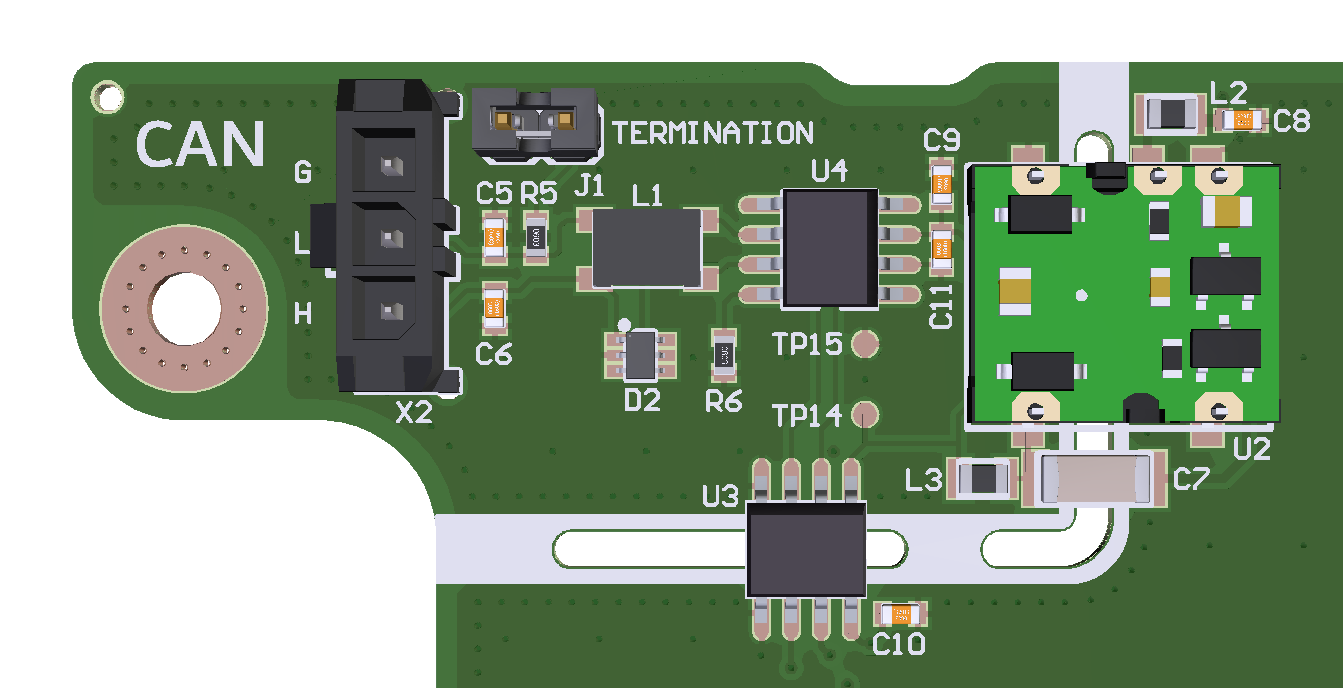
\includegraphics[height=4.5cm]{images/can-pcb}
	\caption{PCB view of CAN interface}
	\vspace{-1.4ex}
	\label{fig:can-pcb}
\end{figure}

\subsubsection{Filter}
A common mode choke as well as bypass capacitors were added to the differential signal lines. A common mode choke is an electrical filter that blocks high frequency noise common to two or more data or power lines while allowing the desired DC or low-frequency signal to pass. Common mode (CM) noise is typically radiated from sources such as radio signals, unshielded electronics, inverters and motors. Additionally matching capacitors on the CANH and CANL lines were added to enhance the immunity against electromagnetic interference. 

\subsubsection{Connector}
The FMS Standard specifies a DIN 72585 connector as the default physical interface. Since these connectors are only available for panel mount, an additional wire to board connector was selected. A Molex \todo{connector name} was chosen because its widely available and being used in lots of applications.\newline

\subsubsection{Termination}
In addition the FMS Standard specifies a 120$\Omega$ CAN termination resistor to be added on the monitor side. To fulfill this requirement and to make it compatible with system that do not need that resistor, a jumper was added to enable/disable the termination.   
\subsection{Accelerometer}
Luca

\newpage
\section{Mechanical Design}
The automotive environment is known for its harsh conditions, such as vibrations, large temperature range and high humidity. The device must withstand those factors and should guarantee a long lifespan. The optimal selection of components, especially the connectors was key to satisfy the requirements and reach an IP67 rating.\newline
As a suitable case for the device, a poly-carbonate watertight enclosure with transparent lid has been chosen. The very robust construction creates an ideal protection for all electronic components.\newline
The case has been machined in the internal workshop of the university. The corresponding mechanical drawings have been made with SolidWorks 2020 and are attached in the appendix: \ref{Fleet-Monitor V1.0 Mechanical Drawing}

\medskip
\begin{figure}[h!]
	\centering
	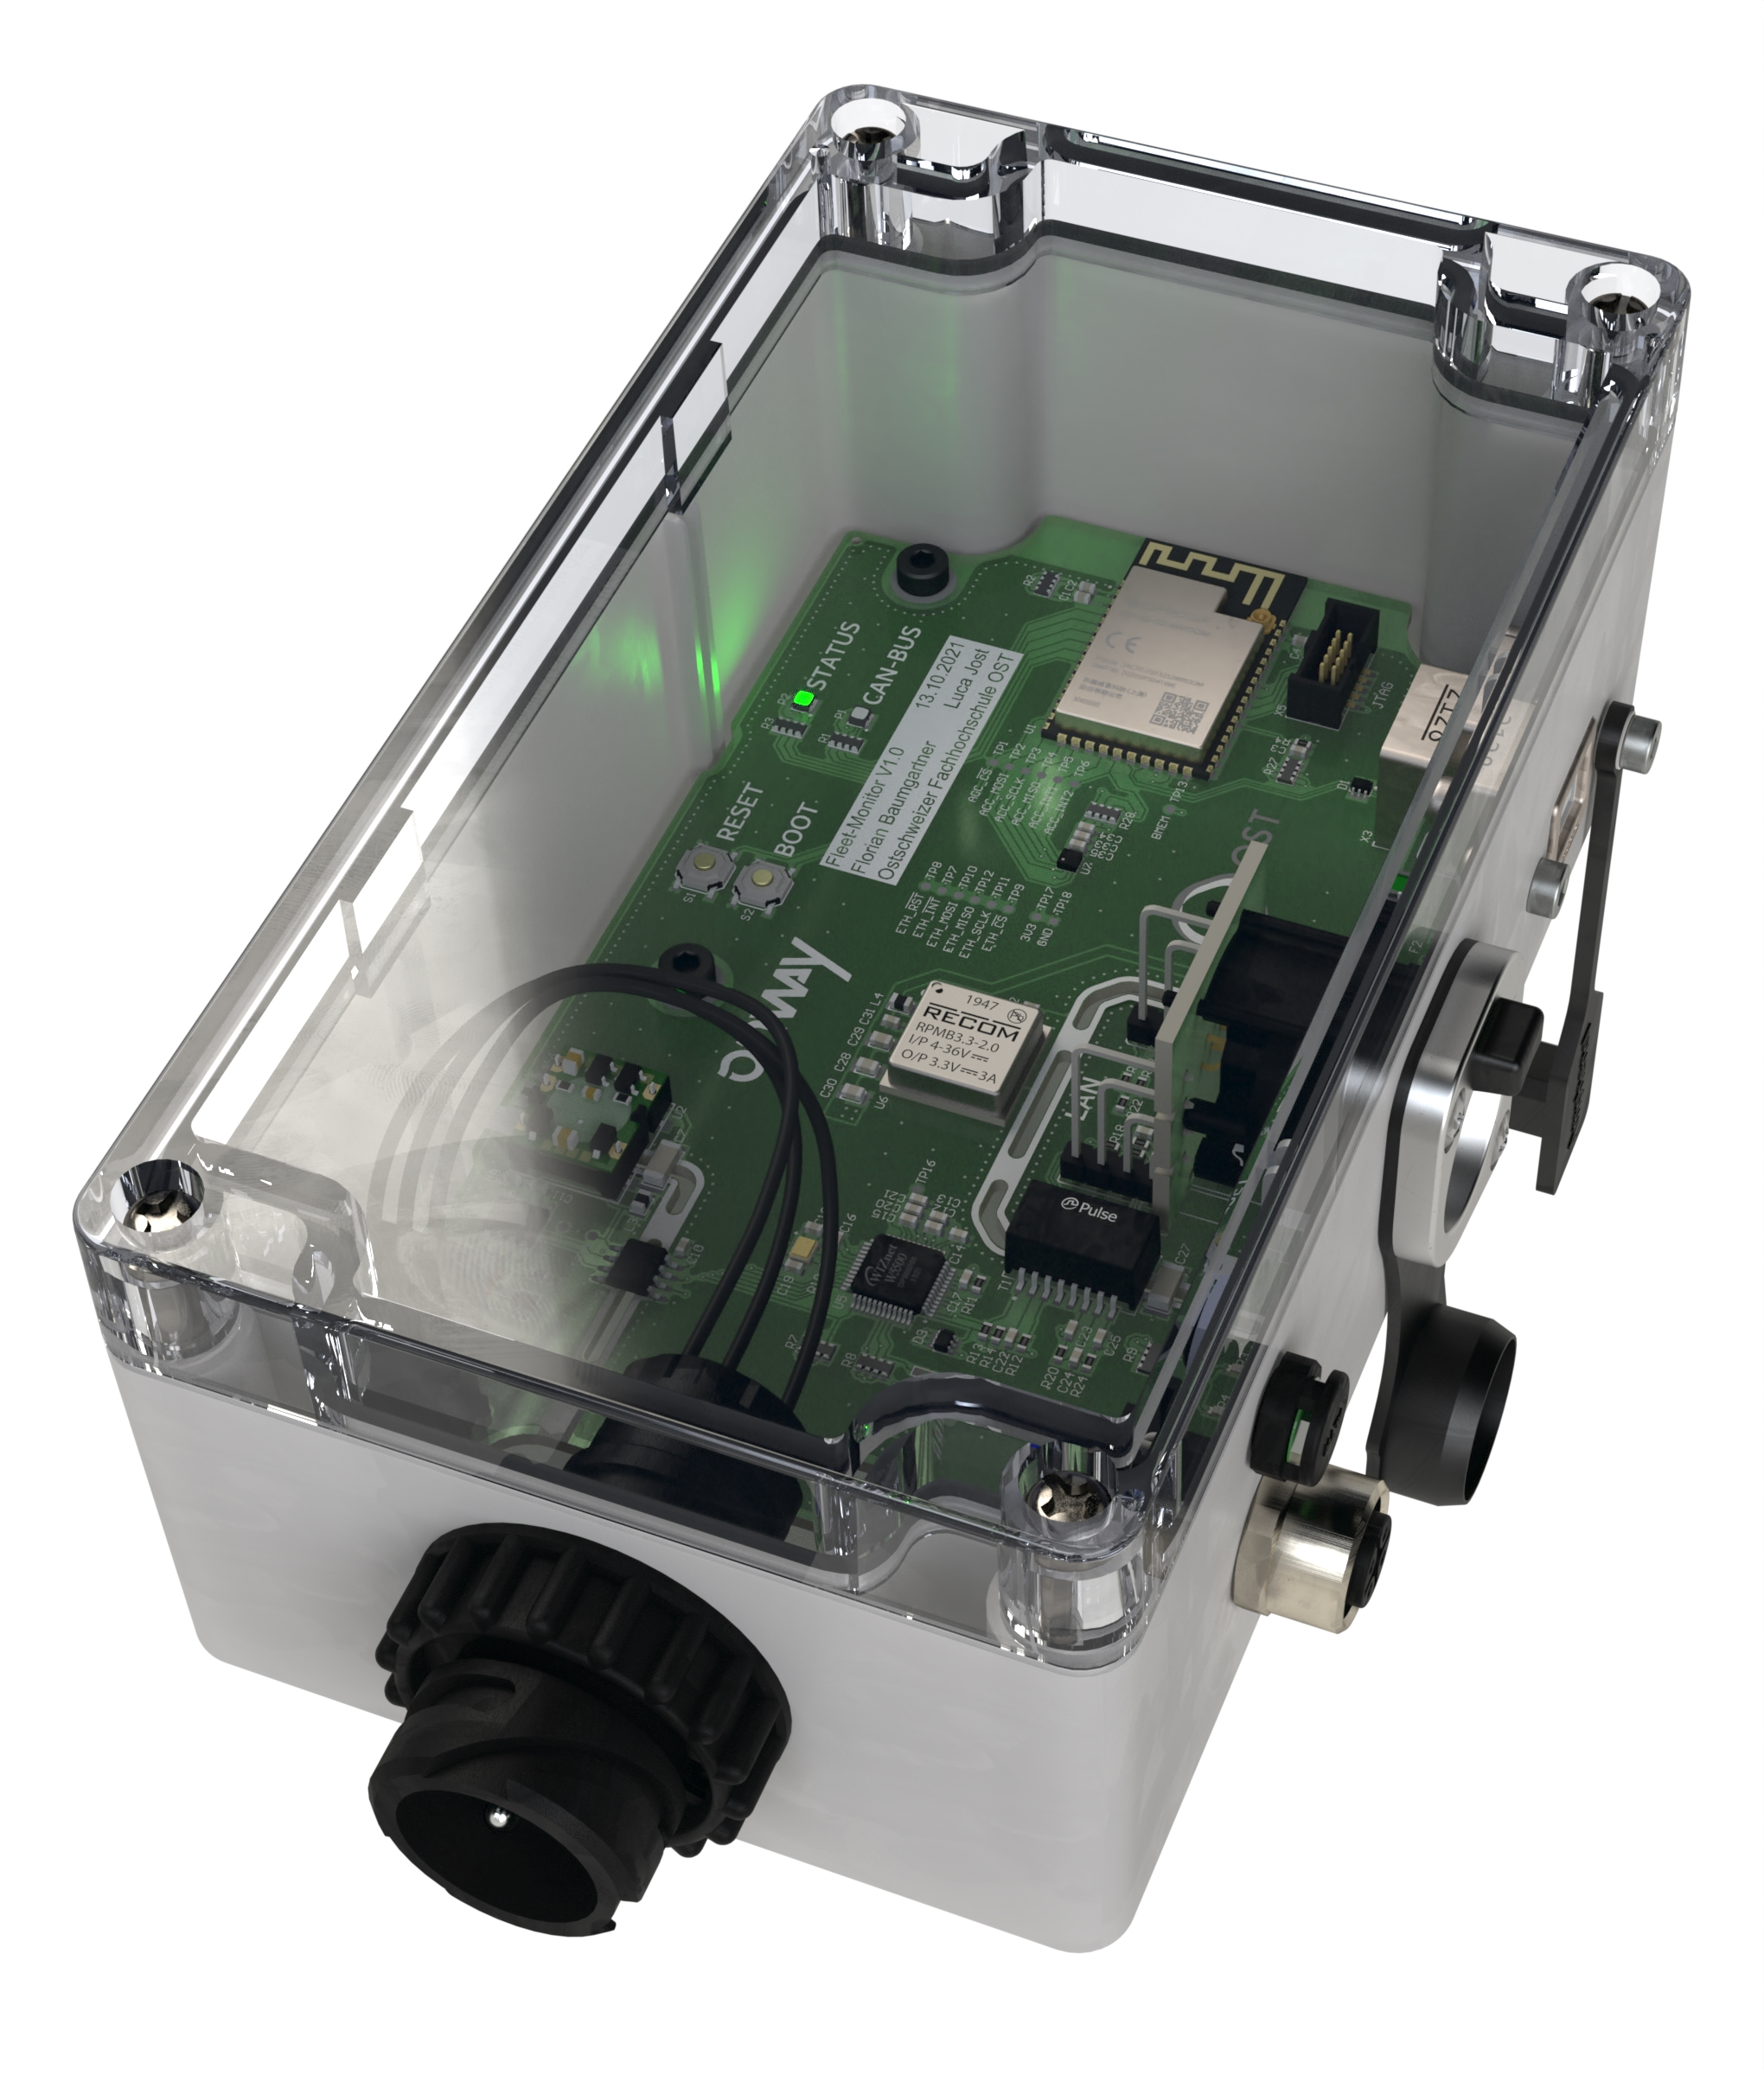
\includegraphics[height=16cm]{images/fleet-monitor-rendering}
	\caption{Final Product 3D-Render}
	\label{fig:fleet-monitor-rendering}
\end{figure}


\newpage
\section{Firmware}
The firmware is written in C++ and is based on a combination of the Arduino and the ESP-IDF framework. As an IDE, Visual Studio Code with PlatformIO as an add-on has been used. This modern environment ensures rapid and effective development.\newline
FreeRTOS has been used as a real time operating system, which guarantees a reliable operation and handles multi-task operations even on a single core system.\newline
The Arduino framework offers extensive library support, especially for the \acrshort{usb} peripheral, file system and Ethernet interface. Due to the large community and the open source licensing, lots of individuals contribute bug-fixes and therefor increase the robustness of the software stack.

\subsection{USB and File system}
The file system is an essential part of the device firmware. It enables accessing files stored on the internal \acrshort{spi}-Flash chip as well as creating an interface for additional libraries.

\medskip
\begin{figure}[h!]
	\centering
	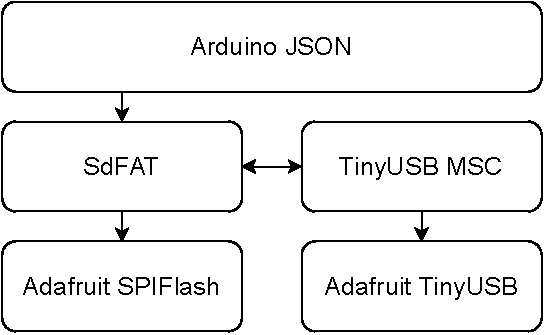
\includegraphics[height=4cm]{images/file_system_stack.pdf}
	\caption{USB and File System Library Stack}
	\label{fig:file_system_stack}
\end{figure}

\colorlet{mygray}{black!30}
\colorlet{mygreen}{green!60!blue}
\colorlet{mymauve}{red!60!blue}
\begin{lstlisting}[backgroundcolor=\color{gray!10},  
                   basicstyle=\ttfamily,
                   columns=fullflexible,
                   breakatwhitespace=false,      
                   breaklines=true,                
                   captionpos=b,                    
                   commentstyle=\color{mygreen}, 
                   extendedchars=true,              
                   frame=single,                   
                   keepspaces=true,             
                   keywordstyle=\color{blue},      
                   language=c++,                 
                   numbers=none,                
                   numbersep=5pt,                   
                   numberstyle=\tiny\color{blue}, 
                   rulecolor=\color{mygray},        
                   showspaces=false,
                   showstringspaces=false,
                   showtabs=false,                 
                   stepnumber=5,                  
                   stringstyle=\color{mymauve},    
                   tabsize=3,                      
                   title=\lstname,
                   frame=none,
                   xleftmargin = 1cm,
                   framexleftmargin = 1em]
utils_init("MONITOR");   // Initialize peripherals and file system
utils_systemConfig("system.json");   // Load system configuration
utils_startMsc();   // Start USB mass storage controller
\end{lstlisting}



\subsubsection{System Configuration}
Florian 
\subsubsection{Frame Configuration}
Florian 

\subsection{Networking}
Luca
\subsubsection{Connection}
Luca
\subsubsection{HTTP}
Luca
\subsection{FMS Frame Handler}
Luca
\subsection{Accelerometer}
Luca

\section{Utility Software Tools}
\subsection{HTTP Server}
Luca
\subsection{FMS Configuration Tool}
Flo
\subsection{FMS Data Visualizer}
Flo
